\documentclass[12pt]{article}

\usepackage[utf8]{inputenc}


\usepackage{caption}
\usepackage{amsmath}
\usepackage{graphicx}
\usepackage{amssymb}
\usepackage{float}
\usepackage{subcaption}\usepackage{multirow}
\usepackage{setspace} \setstretch{0.9}
% set font size to 11pt


\setlength{\parskip}{\baselineskip}%
\setlength{\parindent}{0pt}%


\begin{document}

\title{Spectrum Analysis}
\author{lwp26}
\date{March 2023}
\maketitle

\begin{abstract}
    \centering
    This report analyzed experimental results involving square and triangle waveforms, and an amplitude-modulated sine wave.
    The Fourier coefficients measurements agreed with theory, and the spectrum of the square wave without an anti-aliasing filter was less smooth
    The demodulator circuit parameters were calculated, and test points analysed before and after envelope detection.
    These results confirmed theoretical predictions and demonstrated the circuit's functionality. This study provides insights into circuit implementation and validates theoretical predictions.
\end{abstract}


\section{Introduction}

\subsection{Background}
Spectral analysis is important in signal processing because it allows the frequency content of a signal to be analyzed, which is useful for identifying the physical properties of the signal source. Spectral analysis is used in many areas of science and engineering, such as acoustics, communications, medical imaging, and astronomy, for tasks such as noise reduction, signal filtering, feature extraction, pattern recognition, and data compression.

Amplitude modulation (AM) is a technique used in telecommunications and broadcasting to transmit information by varying the amplitude of a carrier wave. AM is widely used in radio broadcasting, where it allows multiple stations to share the same frequency band and transmit information to a large audience.

\subsection{Aims}

\begin{itemize}
    \item To introduce the concept of spectrum analysis
    \item To become aquainted with the use of simple computer based spectrum analyser software.
    \item To measure the spectra of various simple waveforms.
    \item To study the spectra of amplitude modulated signals and characteristics of a simple demodulator.
\end{itemize}

\section{Theory}

\subsection{Measuring the Spectrum of Signals}

Square and triangle waves can be split into a series of sine and cosine waves at discrete frequencies. The Fourier series of a signal is given by

\begin{equation}
    x(t) = a_0 + \sum_{n=1}^{\infty} a_n \sin(2\pi n f_0 t) + b_n \cos(2\pi n f_0 t)
    \label{eq:1}
\end{equation}

From equation \ref{eq:1} it can see that the Fourier series of a signal is the sum of a constant term, a series of sine terms and a series of cosine terms. 
The terms $a_n$ and $b_n$ are the Fourier coefficients of the signal and signal power at the $n^{th}$ harmonic is given by $P_n = a_n^2 + b_n^2$.

Square wave fourier series
\begin{equation}
    f(t) = \frac{4}{\pi} \sum_{\text{odd n}}^{\infty} \frac{1}{n} \sin\left(n \omega_0 t\right)
    \label{eq:2}
\end{equation}

Triangle wave fourier series
\begin{equation}
    f(t) = \frac{8}{\pi^2} \sum_{\text{odd n}}^{\infty} \pm \frac{1}{n^2} \sin\left(n\omega_0 t\right)
    \label{eq:3}
\end{equation}
where signs alternate, $+$ for $n = 1$

From this it can be seen that the frequency components of the signal decay as $1/n^2$ for the triangle wave and $1/n$ for the square wave. This means that the higher harmonics of the signal have a much smaller amplitude than the lower harmonics.
This should however be expected as a triangle wave can be formed from the convolution of a square pulse and a square wave, which both contain fourier coefficients $1/n$, to give a fourier coefficient containing a $1/n^2$ term.

\subsection{Amplitude Modulation}

Considering a simple information signal $x(t) = E cos(\omega t)$ and a carrier signal $x_c(t) = E_c cos(\omega_0 t)$, the amplitude modulated signal is generated by multiplying the carrier signal with the offsetted information signal as shown below
\begin{equation}
    x_m(t) = E_c(1+m cos(\omega_ct))cos(\omega_0t)
    \label{eq:4}
\end{equation}

Expanding the above gives

\begin{equation}
    x_m(t) = E_c cos(\omega_c t) + \frac{m E_c}{2}cos((\omega_c + \omega_0)t) + \frac{m E_c}{2}cos((\omega_c - \omega_0)t)
    \label{eq:5}
\end{equation}

This shows that the modulated signal has three frequency components, the carrier frequency, the carrier frequency plus the information frequency and the carrier frequency minus the information frequency. The amplitude of the information frequency components is given by $mE_c/2$.

The modulation index can be measured on the frequency spectrum by $m = \frac{2E_c}{E_{fc}} $ where $E_c$ is the frequency component at the carrier frequency and $E_{fc}$ is the frequency component at the carrier frequency plus the information frequency.
The modulation index can also be measured by finding the ratio of maximum and minimum values of the envelope of the modulated signal using eq \ref{eq:6} seen below.
\begin{equation}
    \frac{1+m}{1-m} = \frac{V_{e,max}}{V_{e,min}}
    \label{eq:6}
\end{equation}

\subsection{Amplitude Demodulation}

\begin{figure}[h]
    \centering
    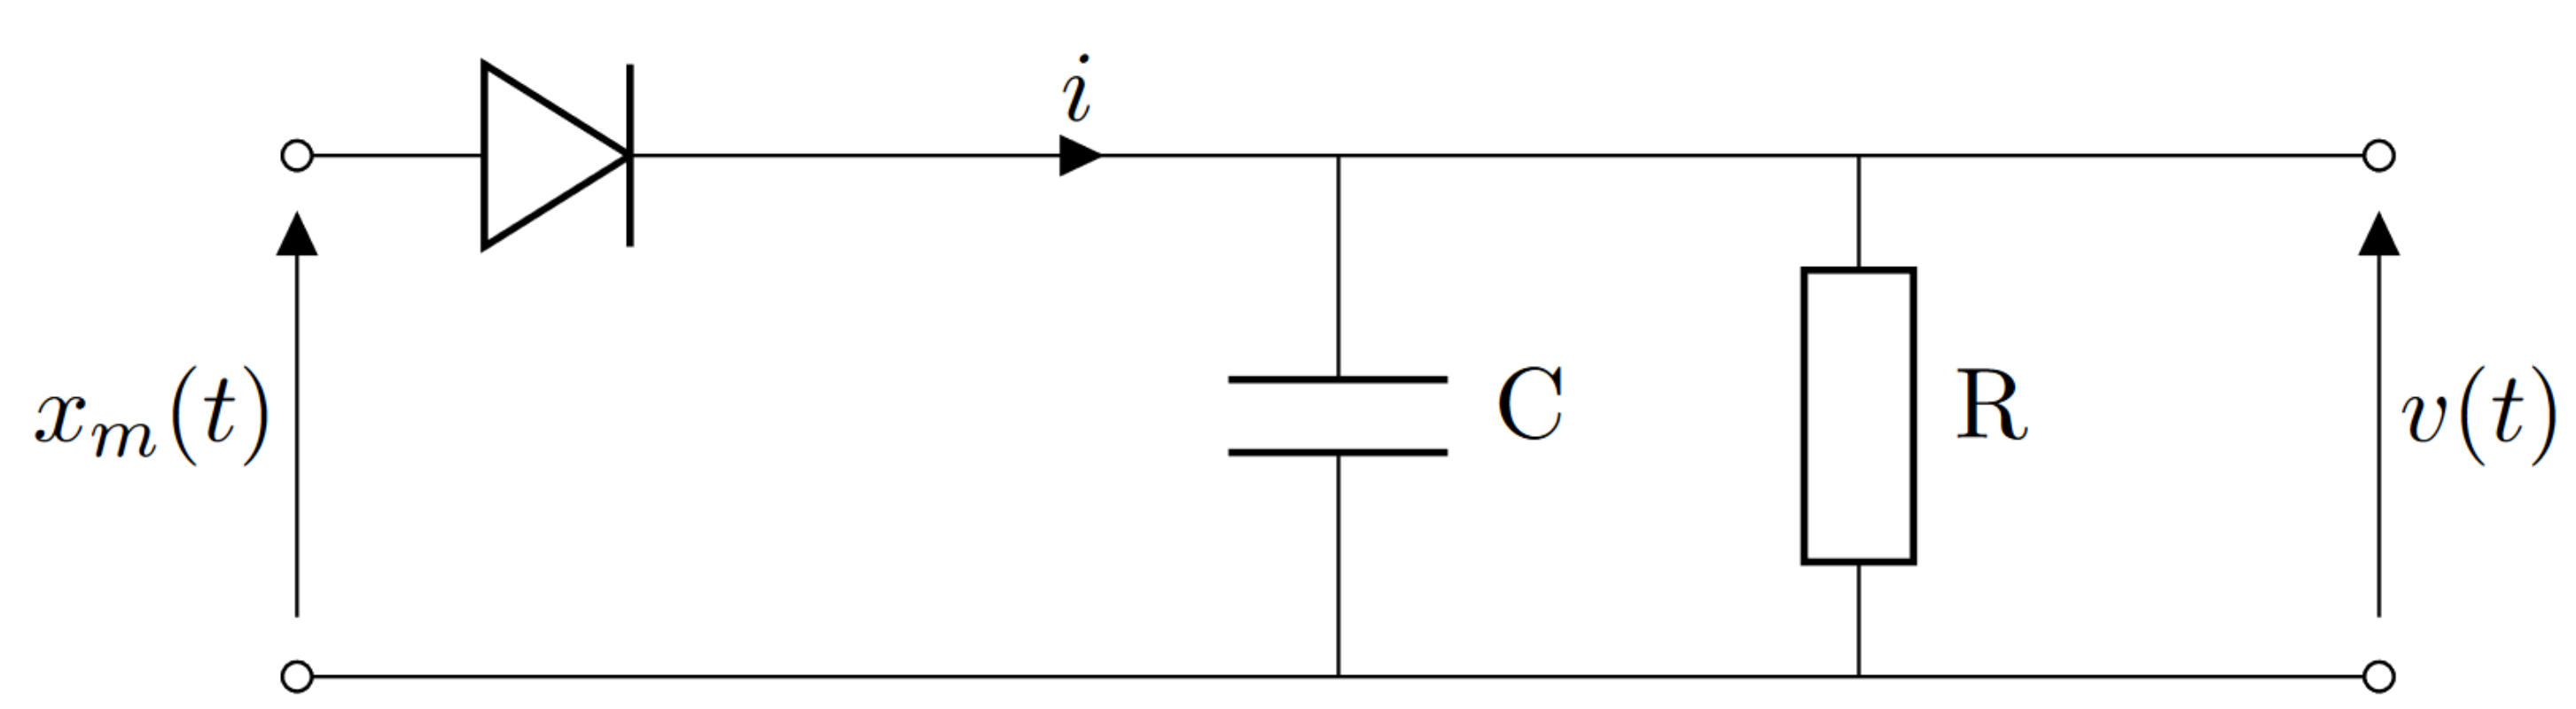
\includegraphics[width=0.8\textwidth]{demod_circuit.png}
    \caption{Demodulator circuit diagram}
    \label{fig:demod_circuit}
\end{figure}

The circuit above shows a simple demodulator circuit and low pass filter.
In the demodulator circuit the step down response from $v_0$ is derived and given as

\begin{equation}
    v(t) = v_0 e^{-\frac{t}{RC}}
    \label{eq:7}
\end{equation}

When we connect a time varying input, $x_m(t)$ the capacitor will alternate
between charging and discharging cycles. During the charging cycle, the capacitor's voltage $v(t)$ will
track the input or $v(t) = xm(t)$. During the discharging cycle, $v(t)$ will decay like Equation \ref{eq:4}. Discharge
will persist until $x_m(t)$ rises to match the falling value of v(t), when the circuit switches to charging.
Charging will end when xm(t) begins to fall again.

Therefor the output of the circuit can be given by

\begin{equation}
    v(t) = 
    \begin{cases}
        v(\tau)e^{-\frac{1}{RC}(t-\tau)}, & \text{if} \ x_m(t) < v(\tau)e^{-\frac{1}{RC}(t-\tau)} \\
        x_m(t), & \text{otherwise}
    \end{cases}
    \label{eq:8}
\end{equation}

\subsection{Apparatus and Setup}

\begin{figure}[h]
    \centering
    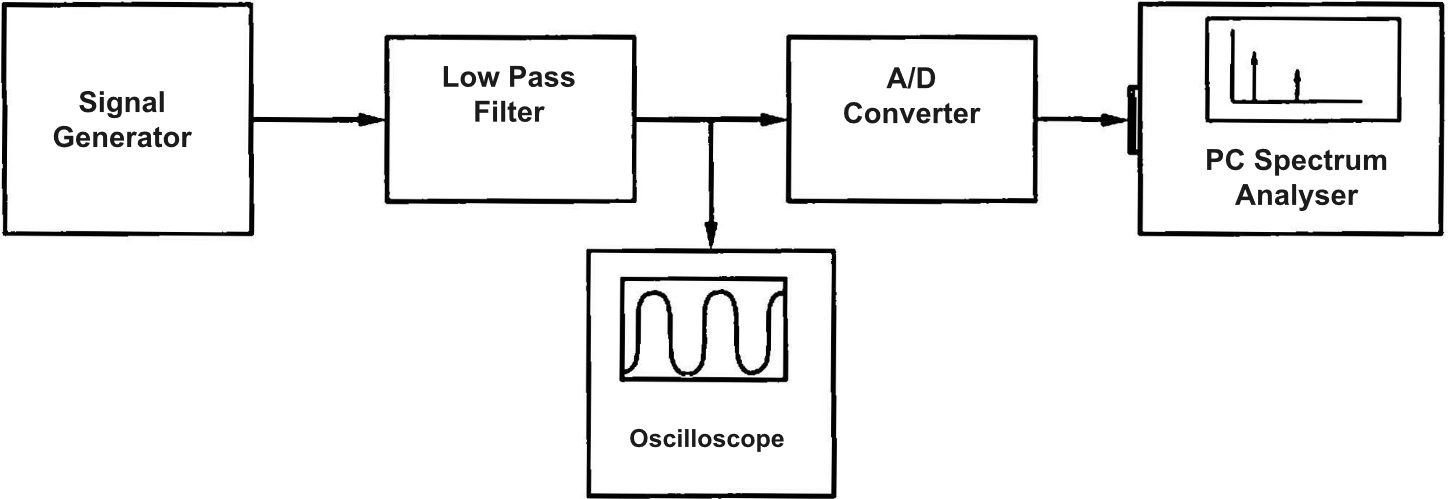
\includegraphics[width=0.8\textwidth]{setup_diagram.png}
    \caption{Graph showing block diagram setup}
    \label{fig:setup}
\end{figure}

This experiment was carried out using a PicoScope as a spectrum analyser using the PicoScope 6 software. The PicoScope was connected to a computer via USB and the PicoScope 6 software was used to display the linear spectrum of the signals.
The signal generator used a chip made by Analog Devices to make precise waveforms.

% add about how the low pass filter or anti aliasing filter was set up, 2khz low pass filter
% add about how the picoscope was set up linear 
\section{Method}
Details on the method and PicoScope settings for each of the data sampled can be found on the lab handout.

\section{Results}

\begin{figure}[H]
    \makebox[\linewidth][c]{%
    \begin{subfigure}[b]{.6\textwidth}
    \centering
    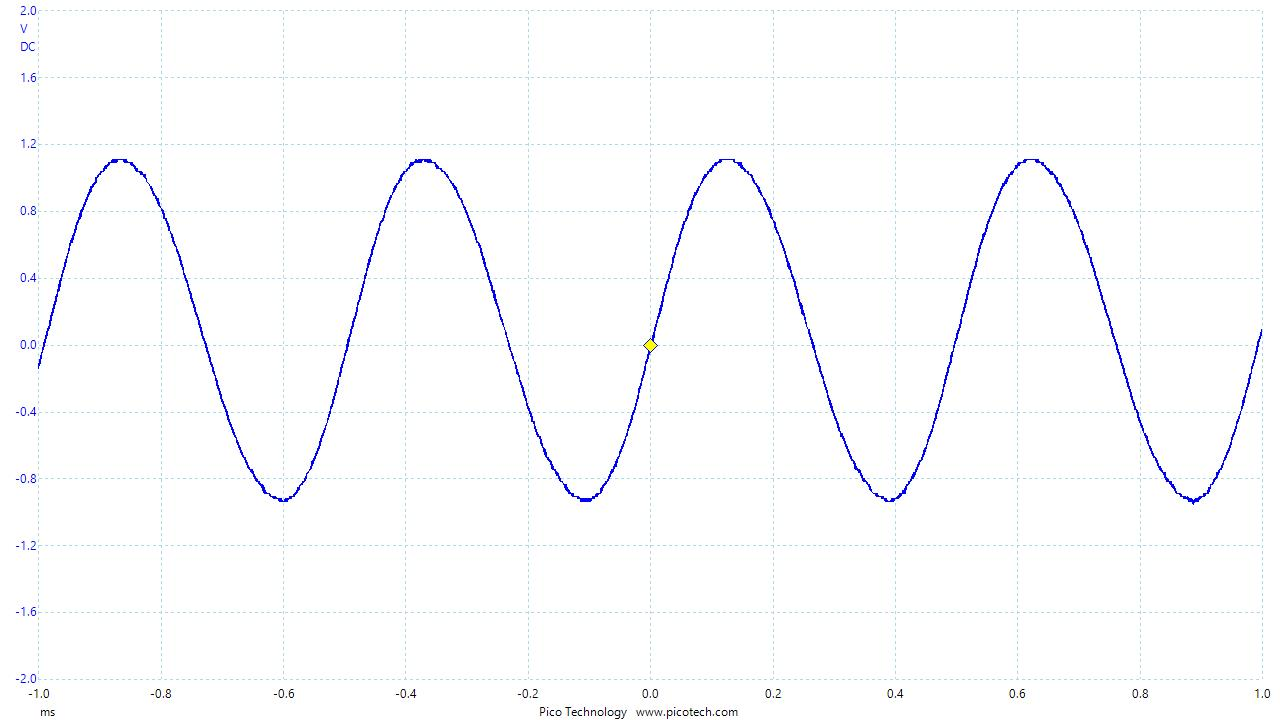
\includegraphics[width=.95\textwidth]{Sine/5kHzSine_t.jpg}
    \caption{Time domain}
    \end{subfigure}%
    \begin{subfigure}[b]{.6\textwidth}
    \centering
    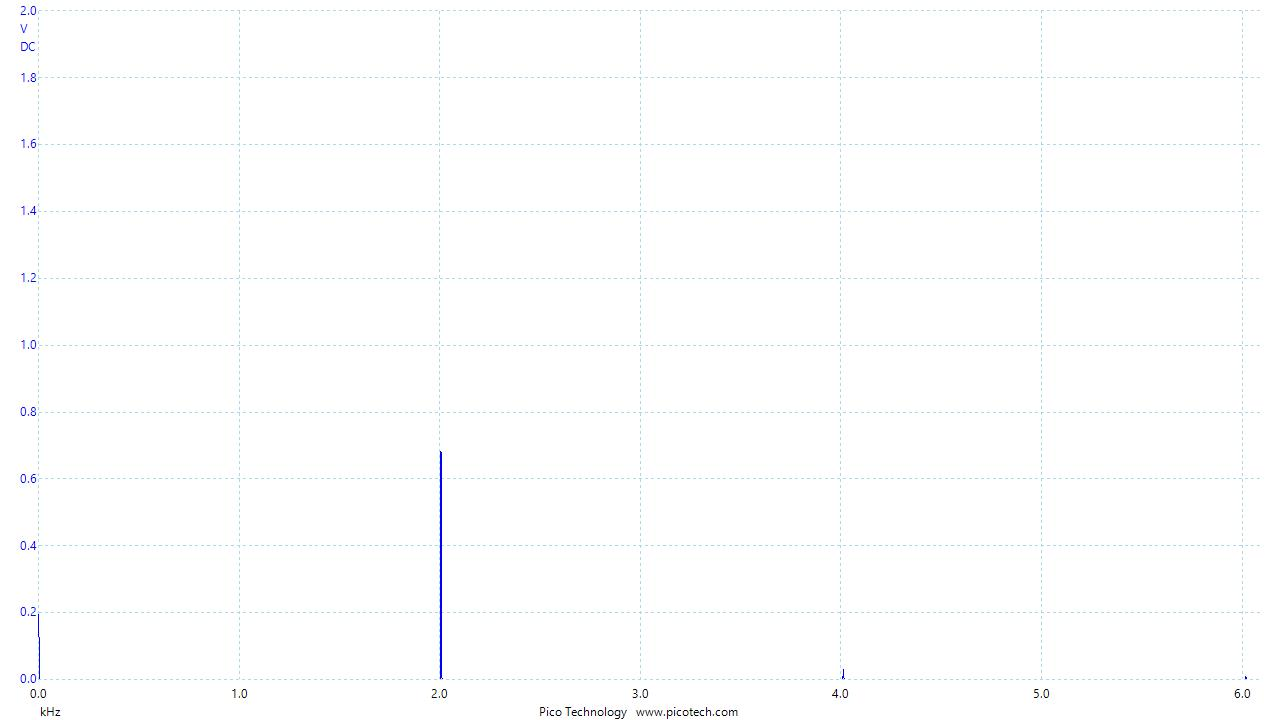
\includegraphics[width=.95\textwidth]{Sine/5kHzSine_f.jpg}
    \caption{Frequency Spectrum}
    \end{subfigure}
    }\\
    \vspace{-14pt}
    \caption{Sine wave with 2kHz anti aliasing filter}
    \label{fig:sine_1khz_filtered}
\end{figure}

\begin{table}[h]
    \centering
    \caption{Frequency composition for Square Wave}
    \begin{tabular}{|c|c|}
    \hline
    Frequency (kHz) & Voltage (mV) \\ \hline
    0.998           & 846.1        \\
    2.998           & 258          \\
    4.995           & 159.6        \\
    6.992           & 98.89        \\
    8.991           & 73.18        \\ \hline
    \end{tabular}
\end{table}

\begin{table}[h]
    \centering
    \caption{Frequency composition for Triangle Wave}
    \begin{tabular}{|c|c|}
    \hline
    Frequency (kHz) & Voltage (mV) \\ \hline
    0.998           & 546.4        \\
    2.992           & 62.9         \\
    4.986           & 22.28        \\
    6.98            & 10.88        \\
    8.987           & 4.895        \\ \hline
    \end{tabular}
\end{table}


\begin{figure}[h]
    \centering
    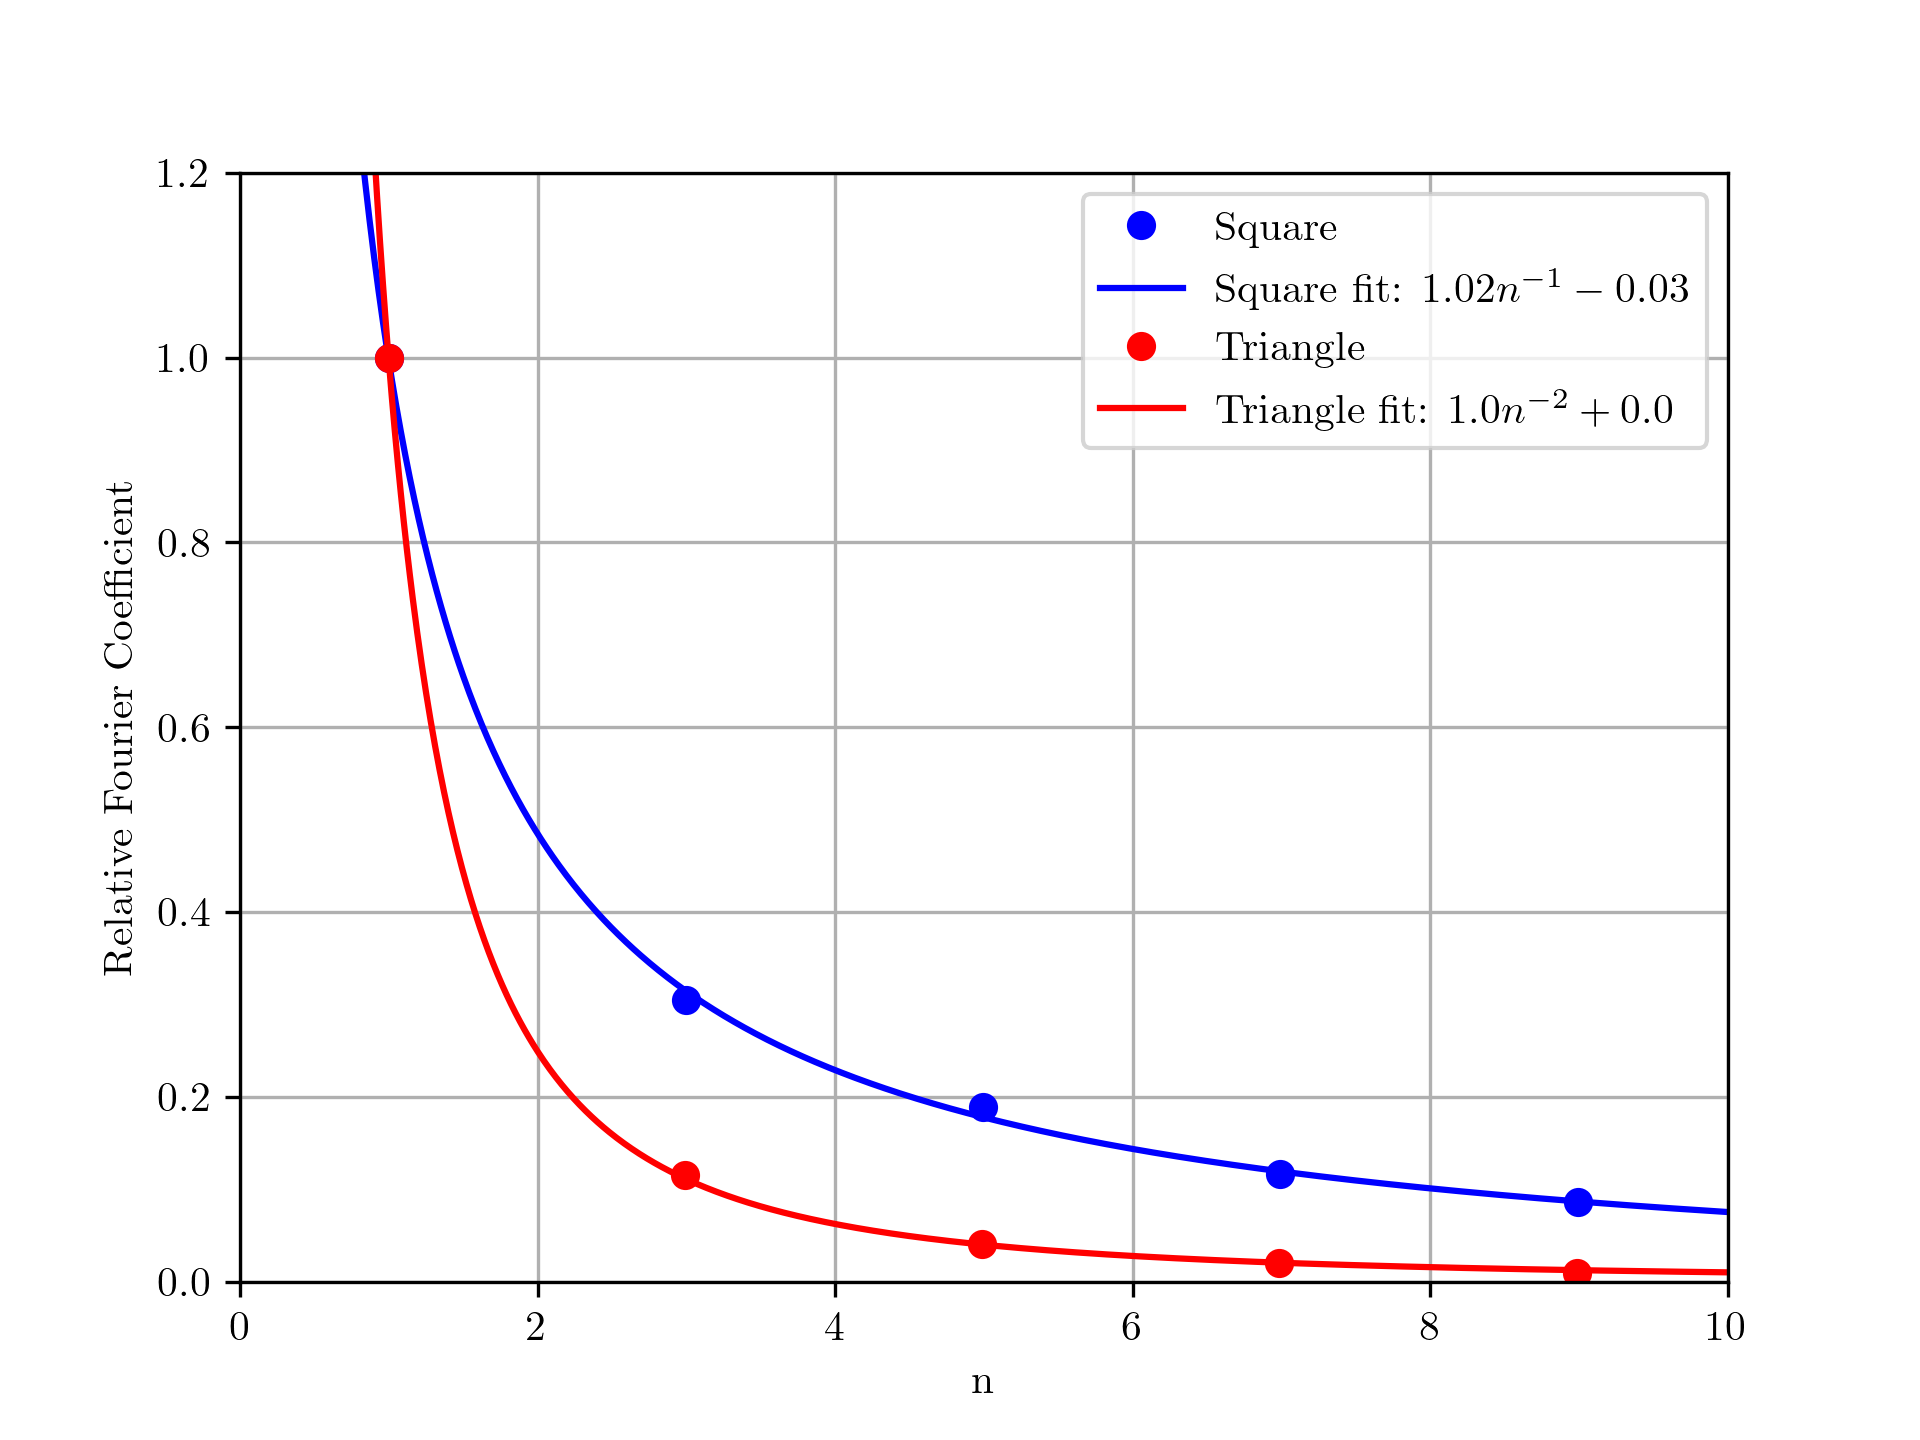
\includegraphics[width=0.8\textwidth]{square_triangle.png}
    \caption{Graph showing measured square and triangle relative fourier coefficients}
    \label{fig:square_triangle}
\end{figure}

\begin{figure}[H]
    \makebox[\linewidth][c]{%
    \begin{subfigure}[b]{.6\textwidth}
    \centering
    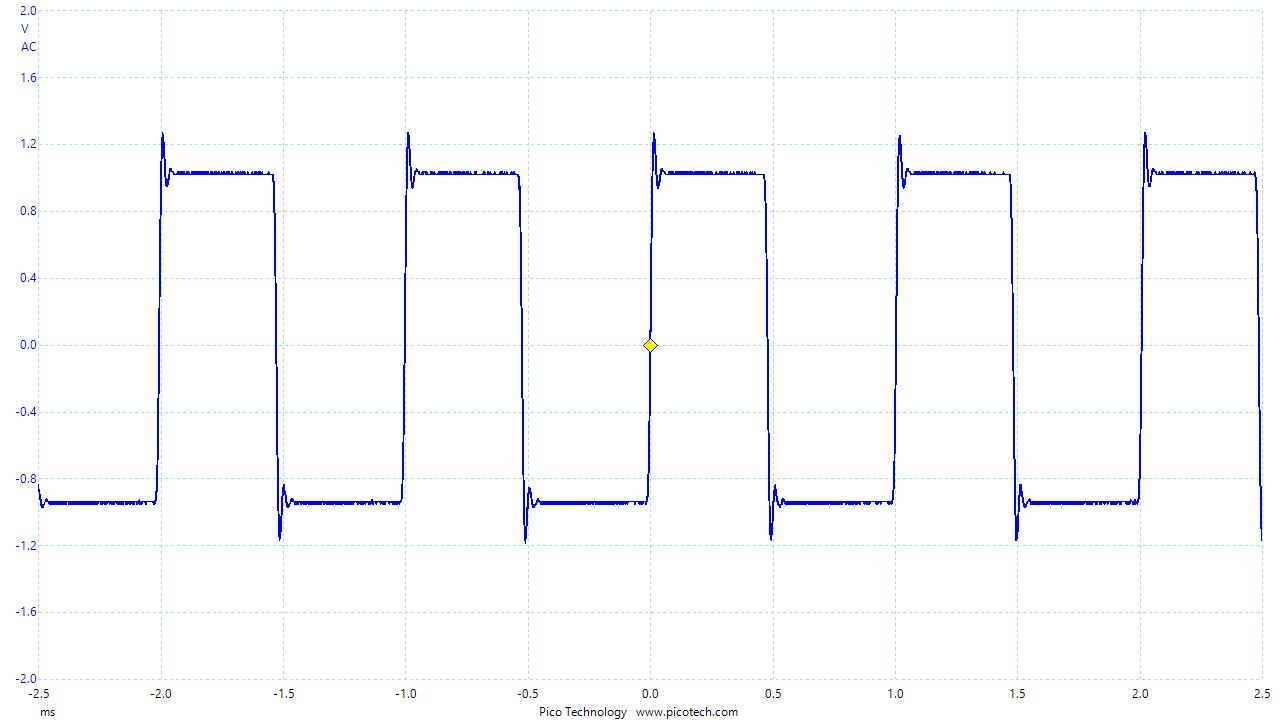
\includegraphics[width=.95\textwidth]{Square/1khzsquare_t.jpg}
    \caption{Time domain}
    \end{subfigure}%
    \begin{subfigure}[b]{.6\textwidth}
    \centering
    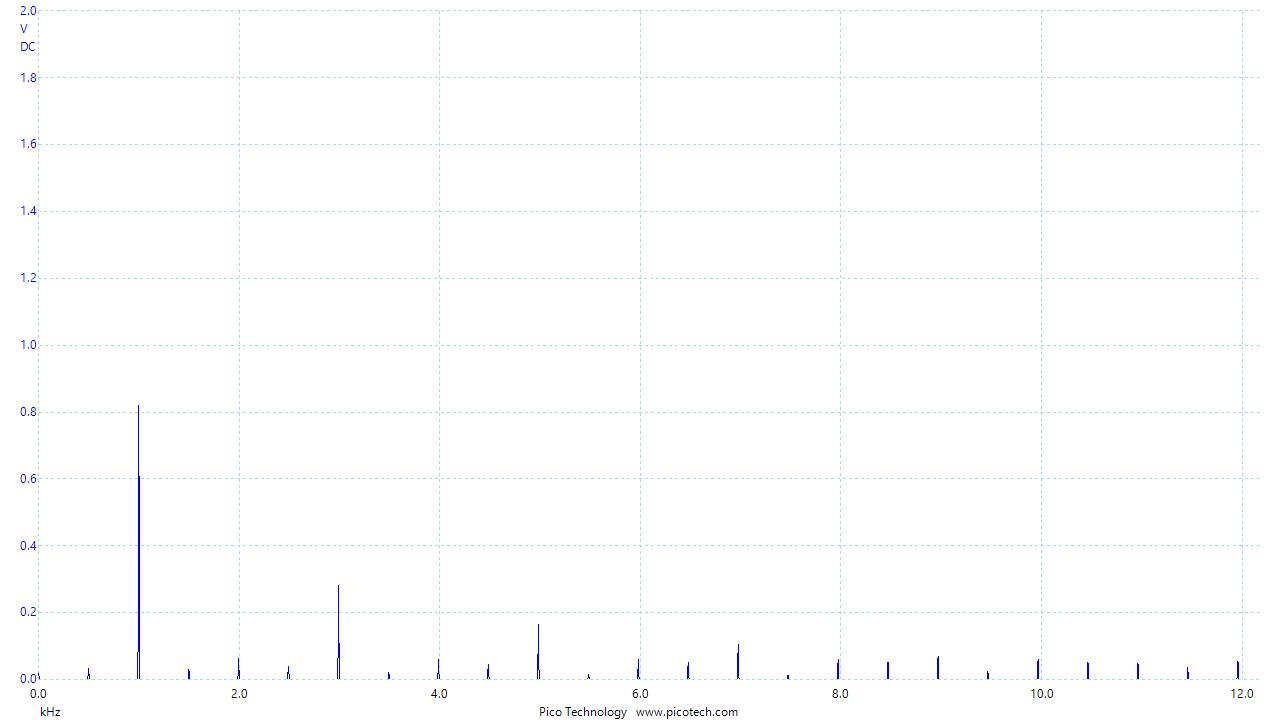
\includegraphics[width=.95\textwidth]{Square/kHzsquare_f.jpg}
    \caption{Frequency Spectrum}
    \end{subfigure}
    }\\
    \vspace{-14pt}
    \caption{Square wave with 2kHz anti aliasing filter}
    \label{fig:square_1khz_filtered}
\end{figure}

\begin{figure}[H]
    \makebox[\linewidth][c]{%
    \begin{subfigure}[b]{.6\textwidth}
    \centering
    \includegraphics[width=.95\textwidth]{Triangle/1khztriangle_t.jpg}
    \caption{Time domain}
    \end{subfigure}%
    \begin{subfigure}[b]{.6\textwidth}
    \centering
    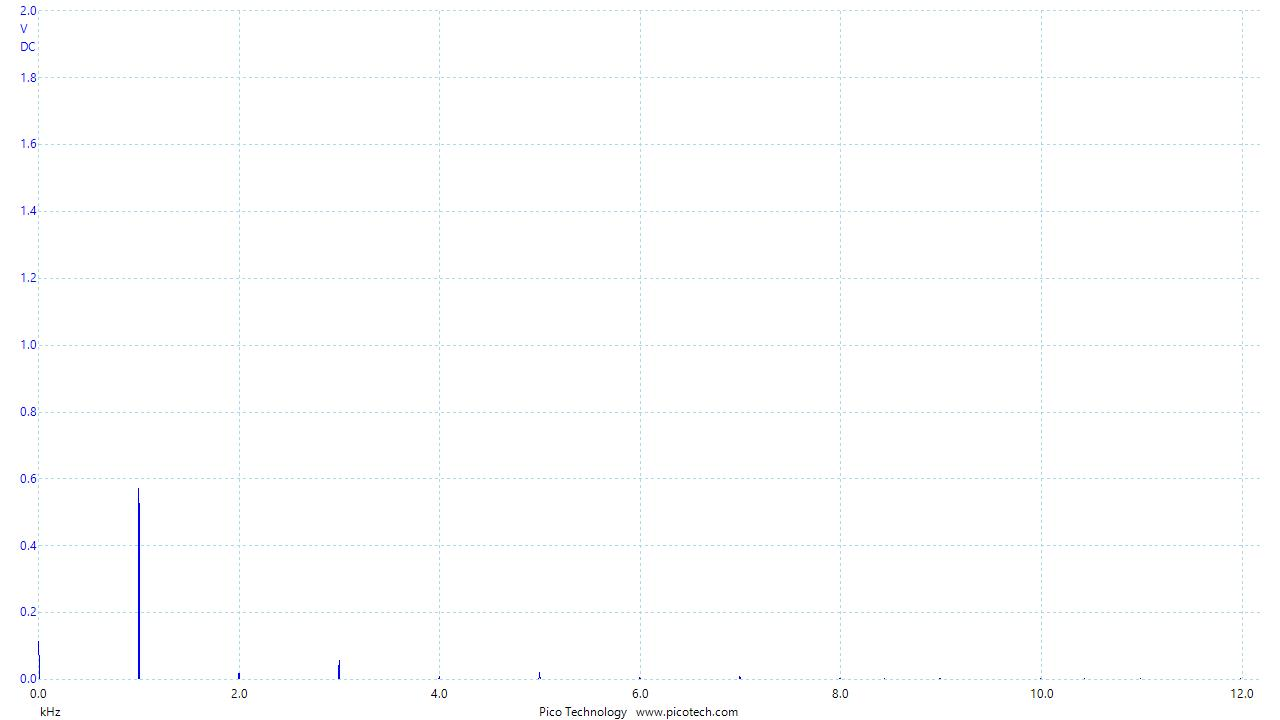
\includegraphics[width=.95\textwidth]{Triangle/1khztriangle_f.jpg}
    \caption{Frequency Spectrum}
    \end{subfigure}
    }\\
    \vspace{-14pt}
    \caption{Triangle wave with 2kHz anti aliasing filter}
    \label{fig:triangle_1khz_filtered}
\end{figure}

\begin{figure}[H]
    \makebox[\linewidth][c]{%
    \begin{subfigure}[b]{.6\textwidth}
    \centering
    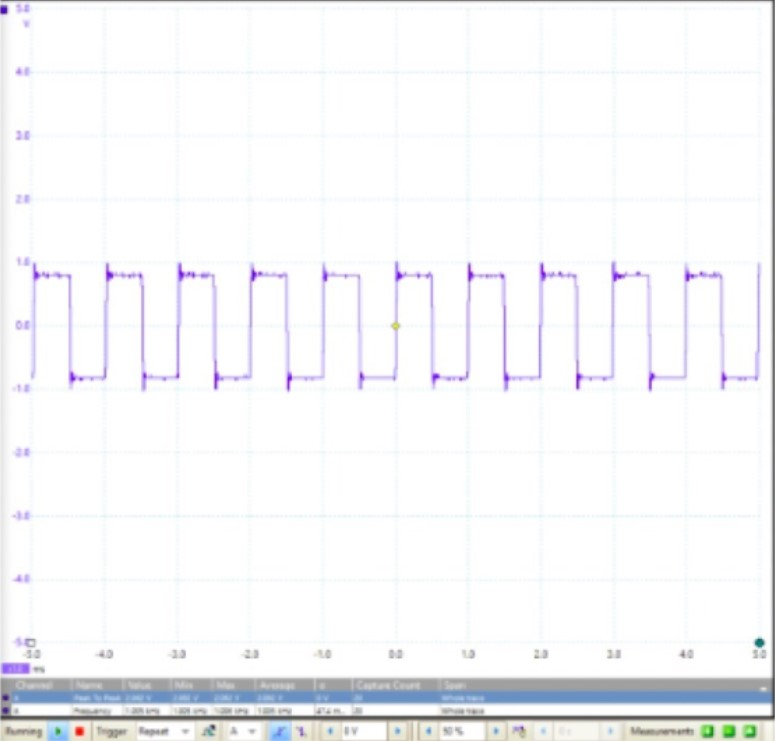
\includegraphics[width=.95\textwidth]{Square/1khzsquare_t_unfiltered.jpg}
    \caption{Time domain}
    \end{subfigure}%
    \begin{subfigure}[b]{.6\textwidth}
    \centering
    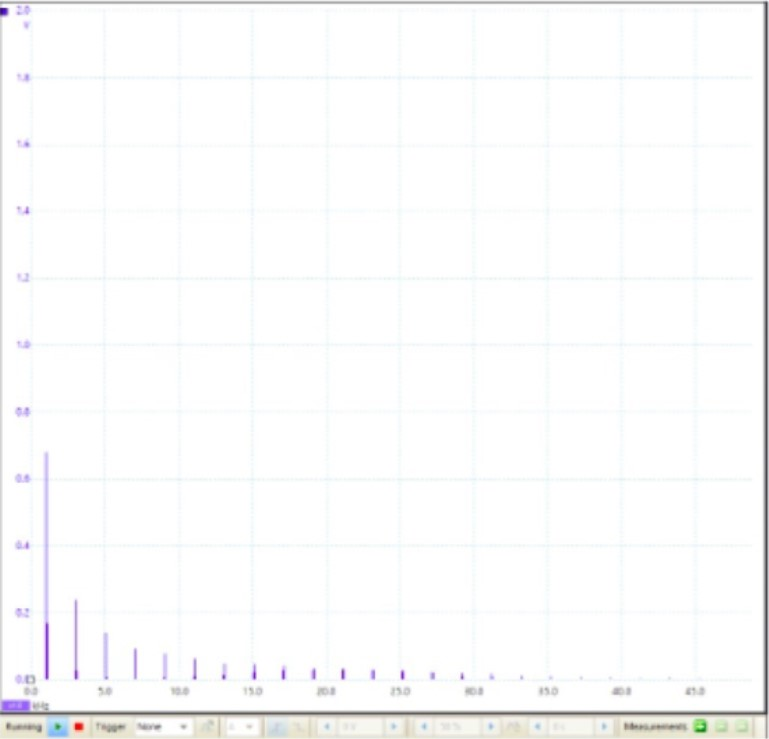
\includegraphics[width=.95\textwidth]{Square/kHzsquare_f_unfiltered.jpg}
    \caption{Frequency Spectrum}
    \end{subfigure}
    }\\
    \vspace{-14pt}
    \caption{Square without anti aliasing filter}
    \label{fig:square_1khz_unfiltered}
\end{figure}

\begin{figure}[H]
    \makebox[\linewidth][c]{%
    \begin{subfigure}[b]{.6\textwidth}
    \centering
    \includegraphics[width=.95\textwidth]{ampmod_t.jpg}
    \caption{Time domain}
    \end{subfigure}%
    \begin{subfigure}[b]{.6\textwidth}
    \centering
    \includegraphics[width=.95\textwidth]{ampMod_f.jpg}
    \caption{Frequency Spectrum}
    \end{subfigure}
    }\\
    \vspace{-14pt}
    \caption{1kHz sine wave modulated with 8kHz carrier with with $m<1$}
    \label{fig:Amplitude_Modulated_Signal}
\end{figure}

\begin{figure}[H]
    \makebox[\linewidth][c]{%
    \begin{subfigure}[b]{.6\textwidth}
    \centering
    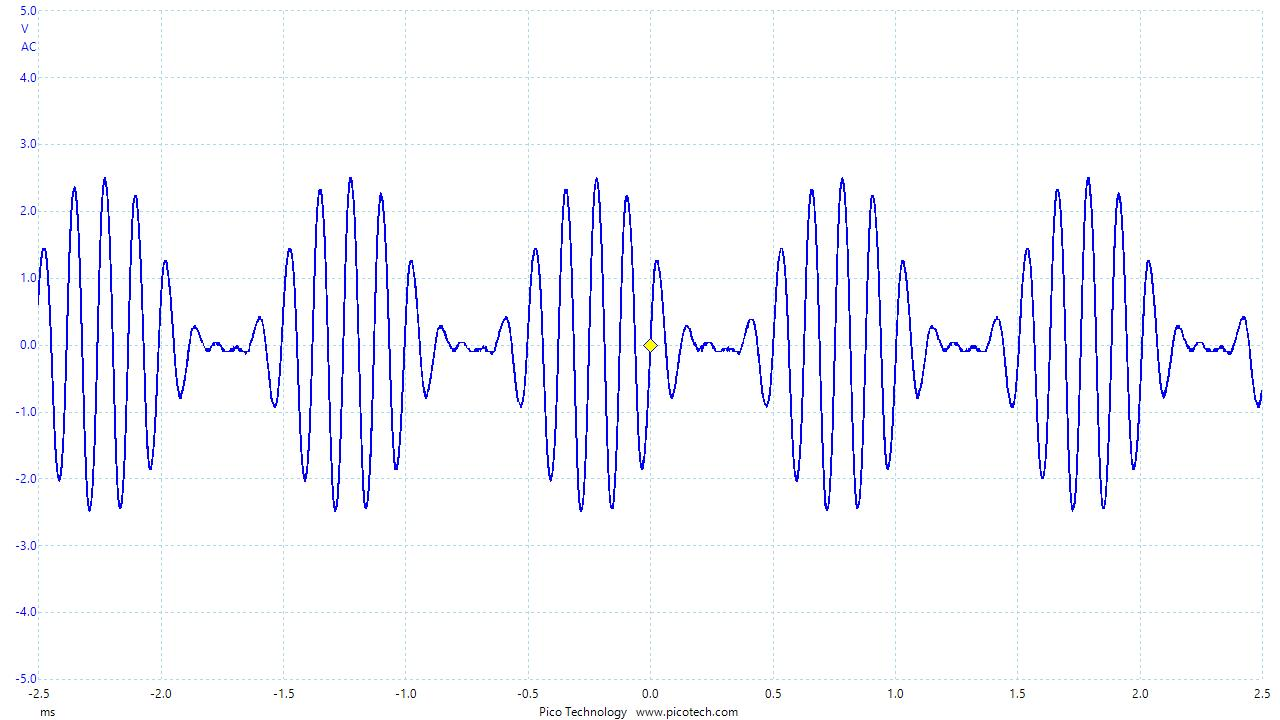
\includegraphics[width=.95\textwidth]{ampModm1_t.jpg}
    \caption{Time domain}
    \end{subfigure}%
    \begin{subfigure}[b]{.6\textwidth}
    \centering
    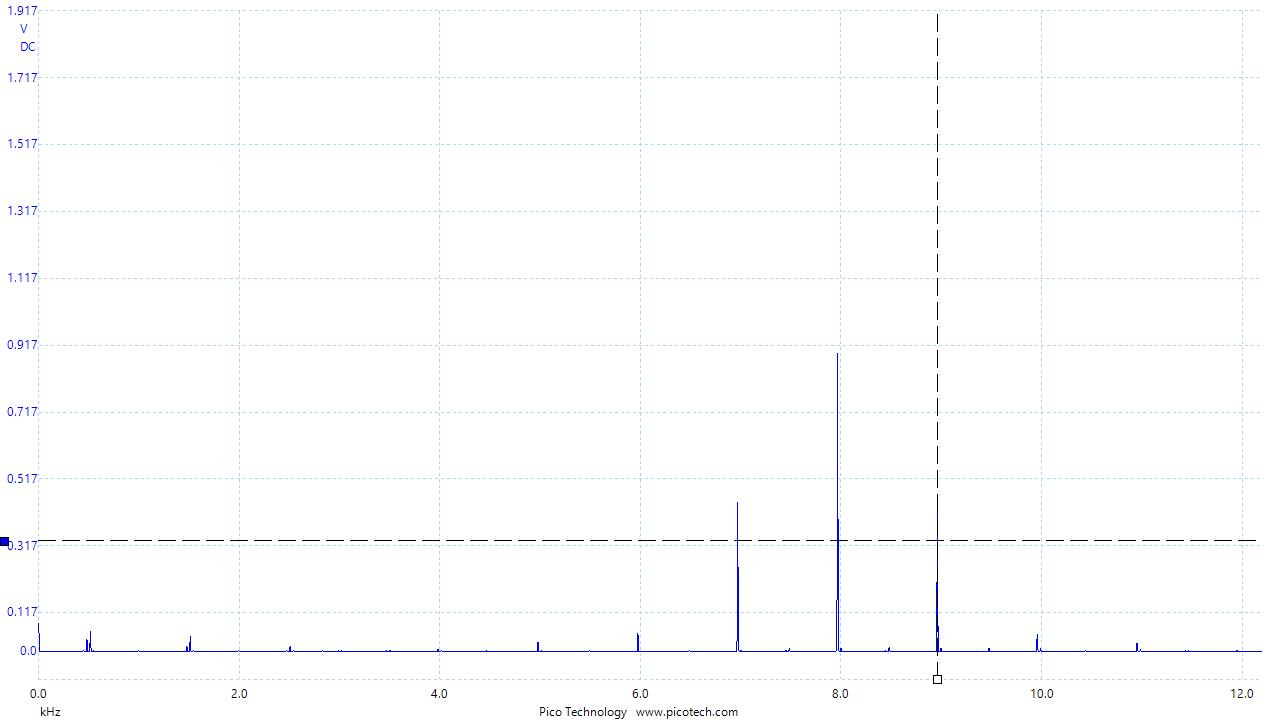
\includegraphics[width=.95\textwidth]{ampModm1_f.jpg}
    \caption{Frequency Spectrum}
    \end{subfigure}
    }\\
    \vspace{-14pt}
    \caption{1kHz sine wave modulated with 8kHz carrier with $m=1$}
    \label{fig:Amplitude_Modulated_Signal_M_1}
\end{figure}

\begin{center}
    \captionof{table}{Amplitudes and modulation index for amplitude modulated signal}
    \begin{tabular}{|c|c|c|c|c|}
    \hline
    $V_{e,max}$ & $V_{e,min}$ & $\frac{1+m}{1-m}$ & $m$ \\
    mV & mV & - & - \\
    \hline 
    $2.611$& $423.5$ & $6.165$ & $0.7212$ \\
    \hline
    \end{tabular}
    \label{tab:3}
\end{center}

The modulation index was also calculated using adjacent frequency components of the spectrum.
By this method the modulation index was found to be $m=0.658$.

\begin{figure}[h]
    \centering
    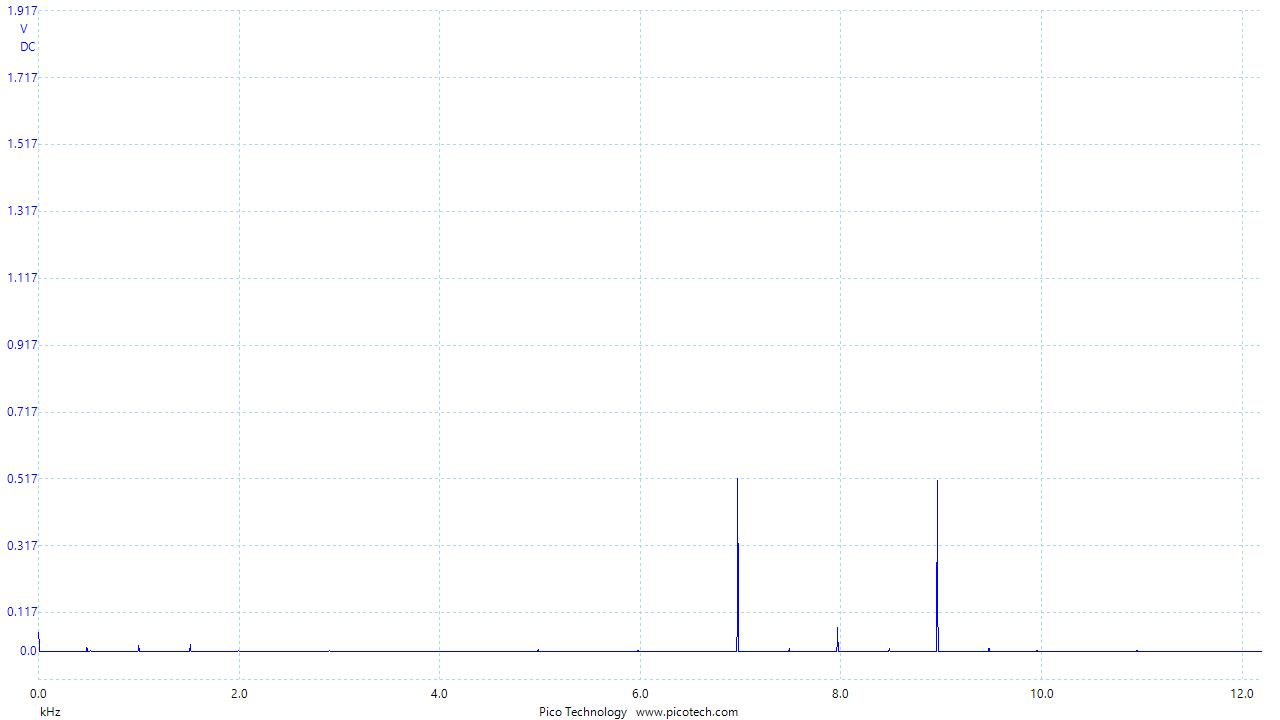
\includegraphics[width=0.8\textwidth]{ampMod_carriermin_f.jpg}
    \caption{Graph showing modulated signal with carrier frequency at minimum}
    \label{fig:freq_responses}
\end{figure}

\begin{figure}[H]
    \makebox[\linewidth][c]{%
    \begin{subfigure}[b]{.6\textwidth}
    \centering
    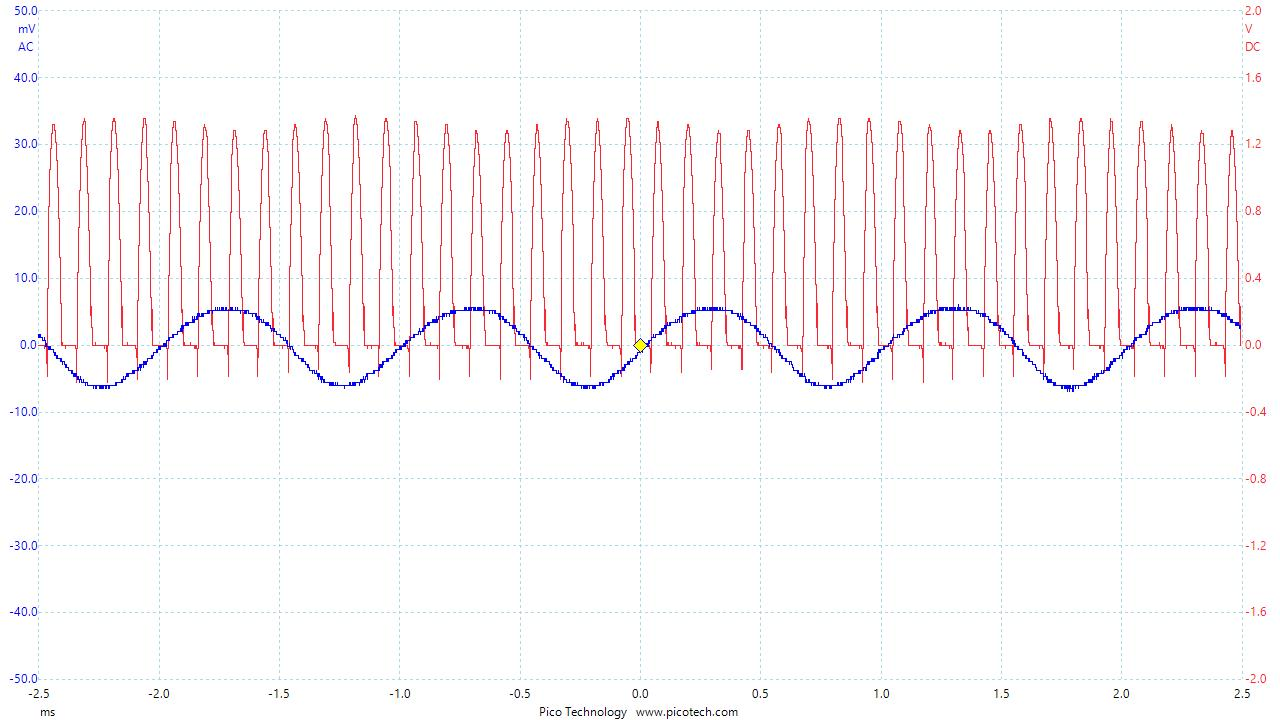
\includegraphics[width=.95\textwidth]{demod_t_TP1.jpg}
    \caption{Time domain}
    \end{subfigure}%
    \begin{subfigure}[b]{.6\textwidth}
    \centering
    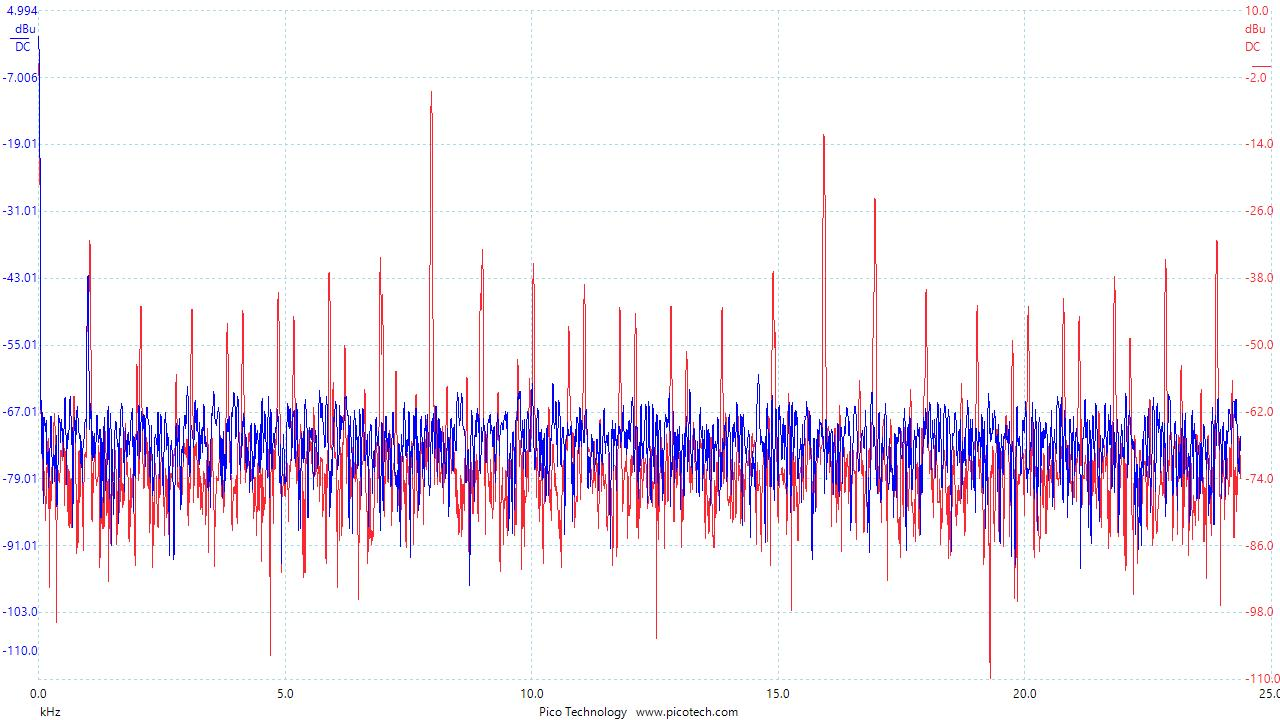
\includegraphics[width=.95\textwidth]{demod_f_TP1.jpg}
    \caption{Frequency Spectrum}
    \end{subfigure}
    }\\
    \vspace{-14pt}
    \caption{Amplitude demodulated signal and Test Point 1 (TP1)}
    \label{fig:Amplitude_Demodulated_Signal_TP1}
\end{figure}

\begin{figure}[H]
    \makebox[\linewidth][c]{%
    \begin{subfigure}[b]{.6\textwidth}
    \centering
    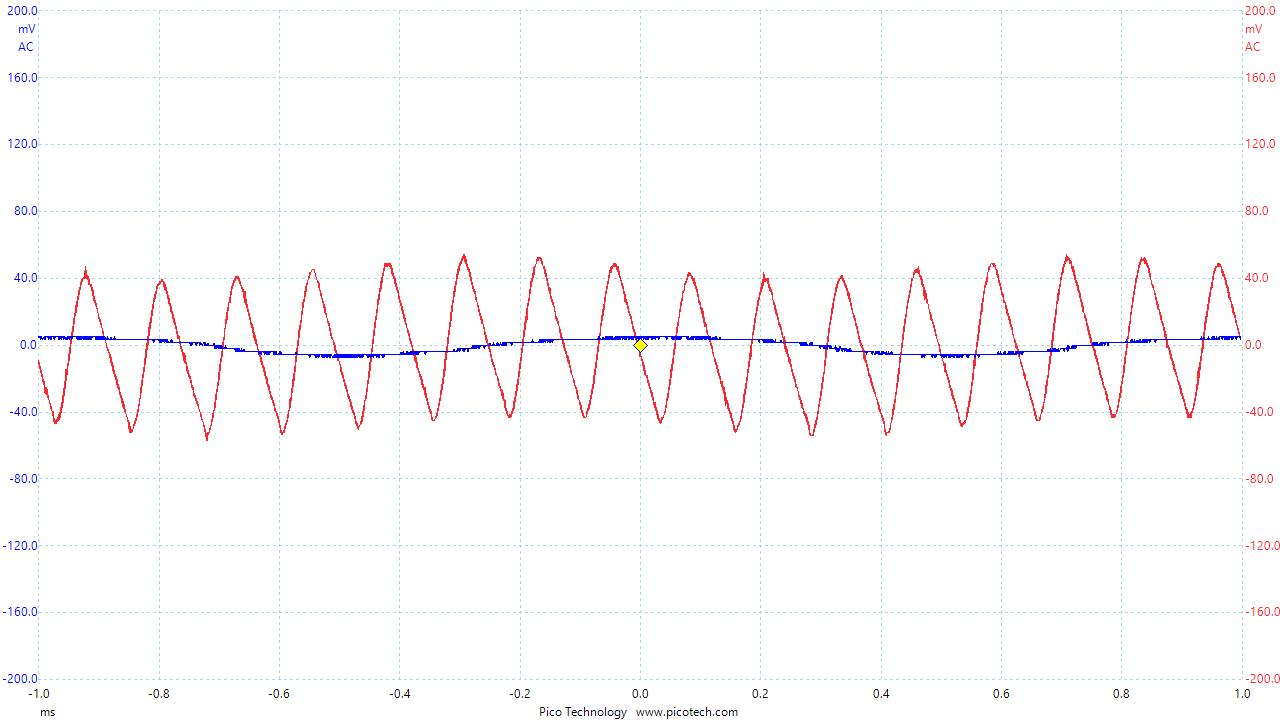
\includegraphics[width=.95\textwidth]{demod_t_TP2.jpg}
    \caption{Time domain}
    \end{subfigure}%
    \begin{subfigure}[b]{.6\textwidth}
    \centering
    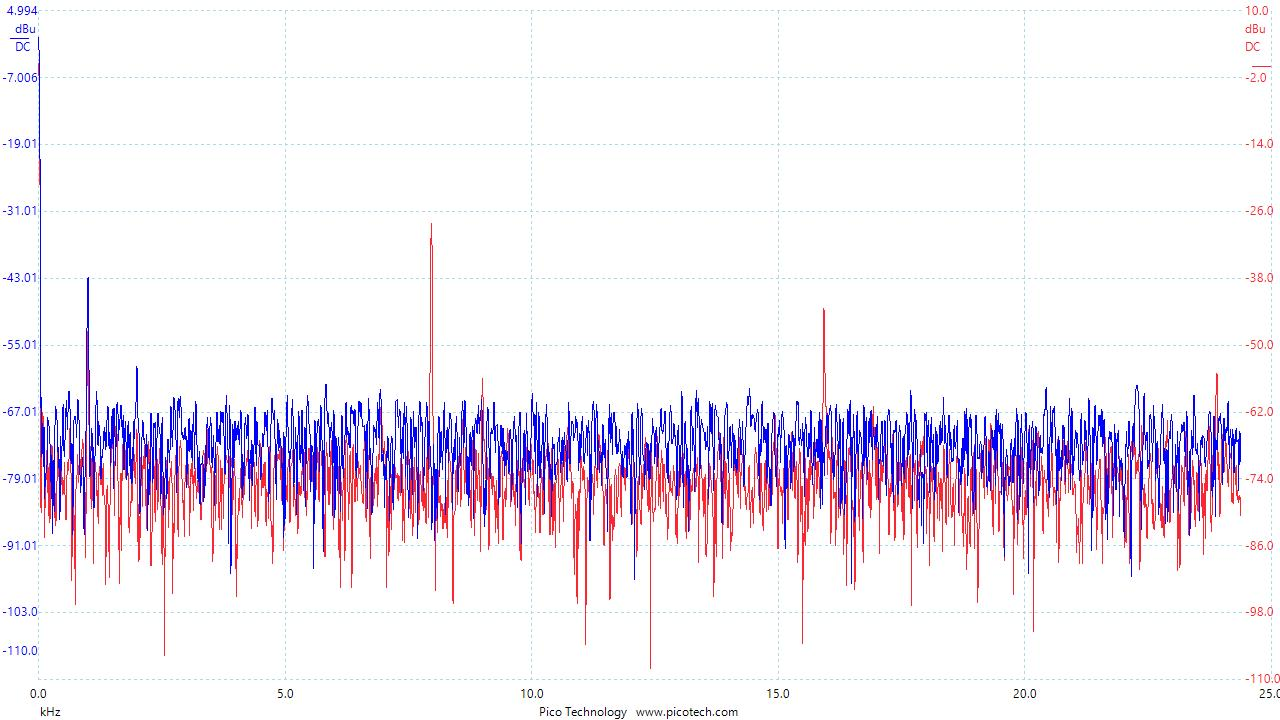
\includegraphics[width=.95\textwidth]{demod_f_TP2.jpg}
    \caption{Frequency Spectrum}
    \end{subfigure}
    }\\
    \vspace{-14pt}
    \caption{Amplitude demodulated signal and Test Point 2 (TP2)}
    \label{fig:Amplitude_Demodulated_Signal_TP2}
\end{figure}

\begin{figure}[h]
    \centering
    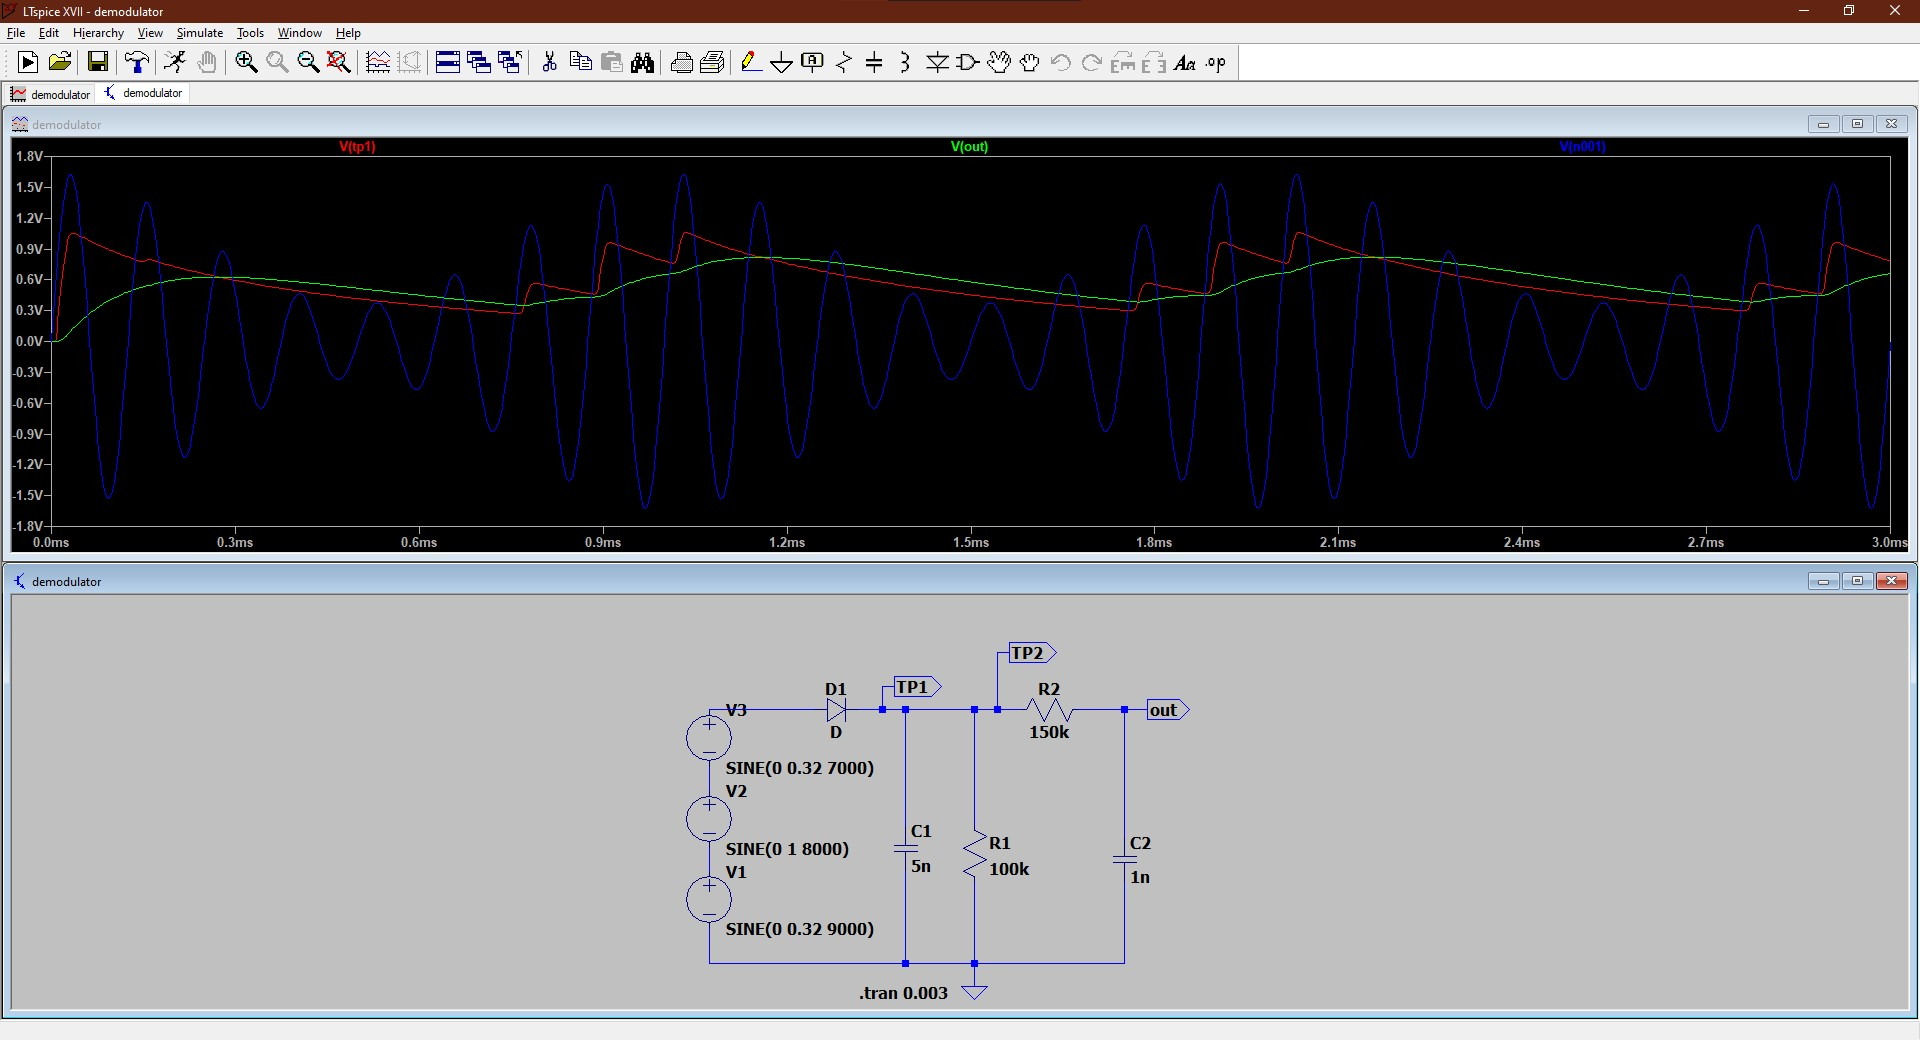
\includegraphics[width=1\textwidth]{LTSpice_circuit/demod_sim.jpg}
    \caption{Demodulator Circuit and Test Points}
    \label{fig:demod_sim}
\end{figure}

\section{Analysis of results}

Square and triangle waveforms
Do your measurements
agree with the theory? If you repeat this exercise without the low-pass/anti-aliasing filter in
the circuit, do you see any differences in the spectrum?

The measurements of fourier coefficients for square and triangle waves agree with the theory.
This is shown by the respective curves fit in Figure \ref{fig:square_triangle} with very tiny adjustments likely due to measurement uncertainty and noise.
The spectrum of the square wave without the anti aliasing filter is shown in Figure \ref{fig:square_1khz_unfiltered}.
On close inspection it can be seen that the spectrum is not as smooth as the spectrum of the square wave with the anti aliasing filter.

The sine wave modulated with a 8kHz carrier seen in Figure \ref{fig:Amplitude_Modulated_Signal} agrees with the theory of shifted frequency components either side of the carrier frequency.
Multiple methods were used to calculate the modulation index of the signal with a difference of 10\% between the two methods.
This difference is significant but likely comes down to the difficulty of measuring the upper and lower envelope amplitudes.
The value is in a valid range $m < 1$ such that $\text{min}_t\{E_c(1+m cos(\omega t))\} > 0$ as when $m=1$ the envelope is no longer bounded.
It can be seen in the envelope of the signal in Figure \ref{fig:Amplitude_Modulated_Signal_M_1} that some of the information signal is cut off and so is lost as expected.

From experimental data circuit parameters can be calculated for the circuit shown in \ref{fig:demod_circuit}.
For the demodulator circuit to work the time constant $RC$ must obey the condition $1/f_c < RC < 1/f_s$ where $f_c$ is the carrier frequency and $f_s$ is the largest fundamental information signal frequency.
The frequency cut off of the low pass filter is the largest fundamental information signal frequency and so the time constant of the low pass can be found by $f_s = \frac{1}{2\pi RC}$.
Using a resistance of $100k\Omega$ for the modulator circuit and $100$ for the demodulator circuit the capacitance of the low pass filter is found to be $C_f=1.06nF$.
The time constant of the demodulator is chosen to be $4/f_c$ which gives a capacitance of $C_m=5nF$.
Test point 1 (TP1) is after the rectifier but before the envelope detection, and TP2 is after the envelope detection.
These can be seen in Figure \ref{fig:Amplitude_Demodulated_Signal_TP1} and \ref{fig:Amplitude_Demodulated_Signal_TP2} respectively.
The simulation agrees with the theoretical predictions, however the experimental results appear to be far smoother.
This is likely due to the demodulator used having a full bridge rectifier and a more sensible choice of time constants for the component values.

\section{Conclusion}
In conclusion, the measurements of Fourier coefficients for square and triangle waveforms agreed with the theory, with only minor adjustments likely due to measurement uncertainty and noise.
The spectrum of the square wave without the anti-aliasing filter showed a less smooth spectrum compared to the square wave with the anti-aliasing filter.
The sine wave modulated with an 8kHz carrier frequency agreed with the theory of shifted frequency components on either side of the carrier frequency, with a modulation index in a valid range.
The demodulator circuit parameters were also calculated, with the time constant of the low pass filter and demodulator chosen to satisfy the condition for the circuit to work.
Overall, the experimental results confirmed the theoretical predictions and demonstrated the functionality of the demodulator circuit.

\end{document}